\documentclass[spanish]{beamer}

%%% CODIFICACIÓN

\usepackage[utf8]{inputenc}
\usepackage[spanish]{babel}
\usepackage{graphics,tikz}
\graphicspath{{./tableros/}}

%%% FUENTES

\usepackage[T1]{fontenc}
\usepackage[familydefault,regular]{}
\usepackage{newtxsf} % Fuente de matemáticas

\setbeamertemplate{navigation symbols}{}

%%% COLORES

\definecolor{background}{RGB}{255,255,255}
\definecolor{text}{RGB}{78,78,78}
\definecolor{accent}{RGB}{6, 105, 125}

\setbeamerfont{framesubtitle}{size=\normalfont\tiny}
\setbeamercolor{framesubtitle}{fg=white}


%%% AJUSTES DE BEAMER

% ¿Negrita en el título de diapositiva o no?
%\setbeamertemplate{frametitle}{\color{accent}\vspace*{1cm}\bfseries\insertframetitle\par\vskip-6pt}

\setbeamertemplate{frametitle}{\color{accent}\vspace*{1cm}\insertframetitle\par\vskip-6pt}

\setbeamertemplate{itemize items}[circle] % Viñetas de itemize

%%% CONFIGURACIÓN DE COLORES DE BEAMER

\setbeamercolor{background canvas}{bg=background}
\setbeamercolor{normal text}{fg=text}
\setbeamercolor{alerted text}{fg=accent}
\setbeamercolor{block title}{fg=accent}
\setbeamercolor{alerted text}{fg=accent}
\setbeamercolor{itemize item}{fg=accent}
\setbeamercolor{enumerate item}{fg=accent}
\setbeamercolor*{title}{fg=accent}
\setbeamercolor{qed symbol}{fg=accent}
\usebeamercolor[fg]{normal text}

%%% TABLAS
\usepackage{longtable}
\usepackage{tabularx}
\usepackage{float}
\usepackage{adjustbox}
\usepackage{booktabs}
\usepackage{multirow}
\usepackage{xcolor,colortbl}
\definecolor{LightCyan}{rgb}{0.88,1,1}
\renewcommand{\arraystretch}{1.7}

%%% Referencias cruzadas HU
\usepackage{xr}
\externaldocument{./Referencias}

%%% INFORMACIÓN DEL DOCUMENTO

\title{Metologías de Desarrollo Ágil : práctica 4}
\subtitle{Plan de entregas iteración 1 y 2}
\author{Miguel Albertí Pons\\ Sofía Almeida Bruno\\ Pedro Manuel Flores Crespo\\ María Victoria Granados Pozo\\ Lidia Martín Chica\vspace{1em}Grupo 2}


\begin{document}

\maketitle

\begin{frame}
\centering
\begin{center}
		
\includegraphics[scale=0.4]{../../Imagenes/Logo}
	\end{center}
\end{frame}

{\small
\begin{frame}[allowframebreaks=0.9]
	\frametitle{Historias de usuario iteración 1}
	\begin{longtable}{p{0.13\linewidth}p{0.65\linewidth}p{0.05\linewidth}p{0.05\linewidth}p{0.05\linewidth}}
		\textbf{HU-\ref{hu:registro}} & Un usuario quiere registrarse en la aplicación para poder planificar su viaje & 2\\
		\textbf{HU-\ref{hu:identificarse}} & Un usuario quiere identificarse en la aplicación para  acceder a su contenido & 1\\
		\textbf{HU-\ref{hu:ver_publicaciones}} & Un usuario quiere ver las publicaciones para saber cuáles le pueden interesar & 2\\
		\textbf{HU-\ref{hu:subir}} & Un usuario quiere subir una publicación para compartir su experiencia & 3\\
		\textbf{HU-\ref{hu:filtrar}.1} & Un usuario quiere filtrar la búsqueda de las publicaciones por lugar & 1/2 \\ 
		\textbf{HU-\ref{hu:filtrar}.2} & Un usuario quiere filtrar la búsqueda de las publicaciones por fecha & 1/2 \\
		\textbf{HU-\ref{hu:filtrar}.3} & Un usuario quiere filtrar la búsqueda de las publicaciones por tipo de publicación (paquete, ruta, actividad, evento) & 1/2 \\
		\textbf{HU-\ref{hu:filtrar}.4} & Un usuario quiere filtrar la búsqueda de las publicaciones por tipo de actividad (cultural, deportiva, etc)) & 1/2 \\
		\textbf{HU-\ref{hu:personalizar}.1} & Un usuario quiere eliminar una actividad de un paquete & 1/2\\ 
		\textbf{HU-\ref{hu:seleccionar}} & Un usuario quiere seleccionar un viaje/actividad para realizarlo & 3/2 \\
	\end{longtable}
\end{frame}
}

\begin{frame}
	\frametitle{Carga de los desarrolladores}
	\begin{table}[H]
	  \centering
	  \begin{adjustbox}{width=\textwidth}
	\begin{tabular}{lrrrrr}
	  \toprule
	  \textbf{Desarrollador} & \textbf{Velocidad inicial} & \textbf{Dedicación} & \textbf{Carga de trabajo} & \textbf{Tareas aceptadas} \\
	  & \textbf{(días ideales)} & \textbf{(\% de tiempo)} & \textbf{(días ideales)} & \textbf{ (cantidad)}\\
	  \midrule
	  MAP & 12 & 60 & 12.5 & 5\\
	  SAB & 12 & 60 & 13 & 13\\
	  PFC & 12 & 60 & 12.5 & 5\\
	  MVGP & 12 & 60 & 13 & 11\\
	  LMC & 12 & 60 & 12.2 & 10\\
	  \bottomrule
	\end{tabular}
	\end{adjustbox}
	\end{table}
\end{frame}

\begin{frame}
	\frametitle{Planificación primera semana}
	\begin{table}[H]
	\begin{adjustbox}{width=\textwidth}
	\begin{tabular}{lrrrrr}
	  \toprule
	  \textbf{Desarrollador} & \textbf{Día 1} & \textbf{Día 2} & \textbf{Día 3} & \textbf{Día 4} \\
	  \midrule
	  MAP  &Tarea 1-1 & & Tarea 2-2 &  \\
	  SAB &   Tarea 1-2  & Tarea 9.1-1, 9.1-3 &  & Tarea 9.2-1\\
	  PMFC &Tarea 1-4 & &Tarea 3-1 \\
	  MVGP & Tarea 1-1 &Tarea 11-1, 11-2 &Tarea 9.2-4 & Tarea 9.1-4 \\
	  LMC & Tarea 1-3 & Tarea 2-1 & Tarea 4-1& Tarea 2-3, 3-3 \\
	  \bottomrule
	\end{tabular}
	\end{adjustbox}
	\end{table}
\end{frame}

\begin{frame}
	\frametitle{Planificación segunda semana}
	\begin{table}[H]
	\begin{adjustbox}{width=\textwidth}
	\begin{tabular}{lrrrrr}
	  \toprule
	  \textbf{Desarrollador} & \textbf{Día 1} & \textbf{Día 2} & \textbf{Día 3} & \textbf{Día 4} \\
	  \midrule
	  MAP &Tarea 3-2  && & Tarea 9.2-2 \\
	  SAB & Tarea 4-2  & Tarea 9.3-2, 9.3-4, 9.4-1 & Tarea 9.4-2, 9.4-5 10-2 \\
	  PMFC & Tarea 4-3 &  &Tarea 11-5 & Tarea 4-5 \\
	  MVGP &Tarea 9.2-3 9.2-4& Tarea 9.4-3, 11-4&Tarea 10-1 & \\
	  LMC  &Tarea 11-3&& Tarea 4-4, 9.3-4, 10-3& Tarea 9.4-5, \\
	  \bottomrule
	\end{tabular}
	\end{adjustbox}
	\end{table}
\end{frame}


\begin{frame}
	\begin{center}
		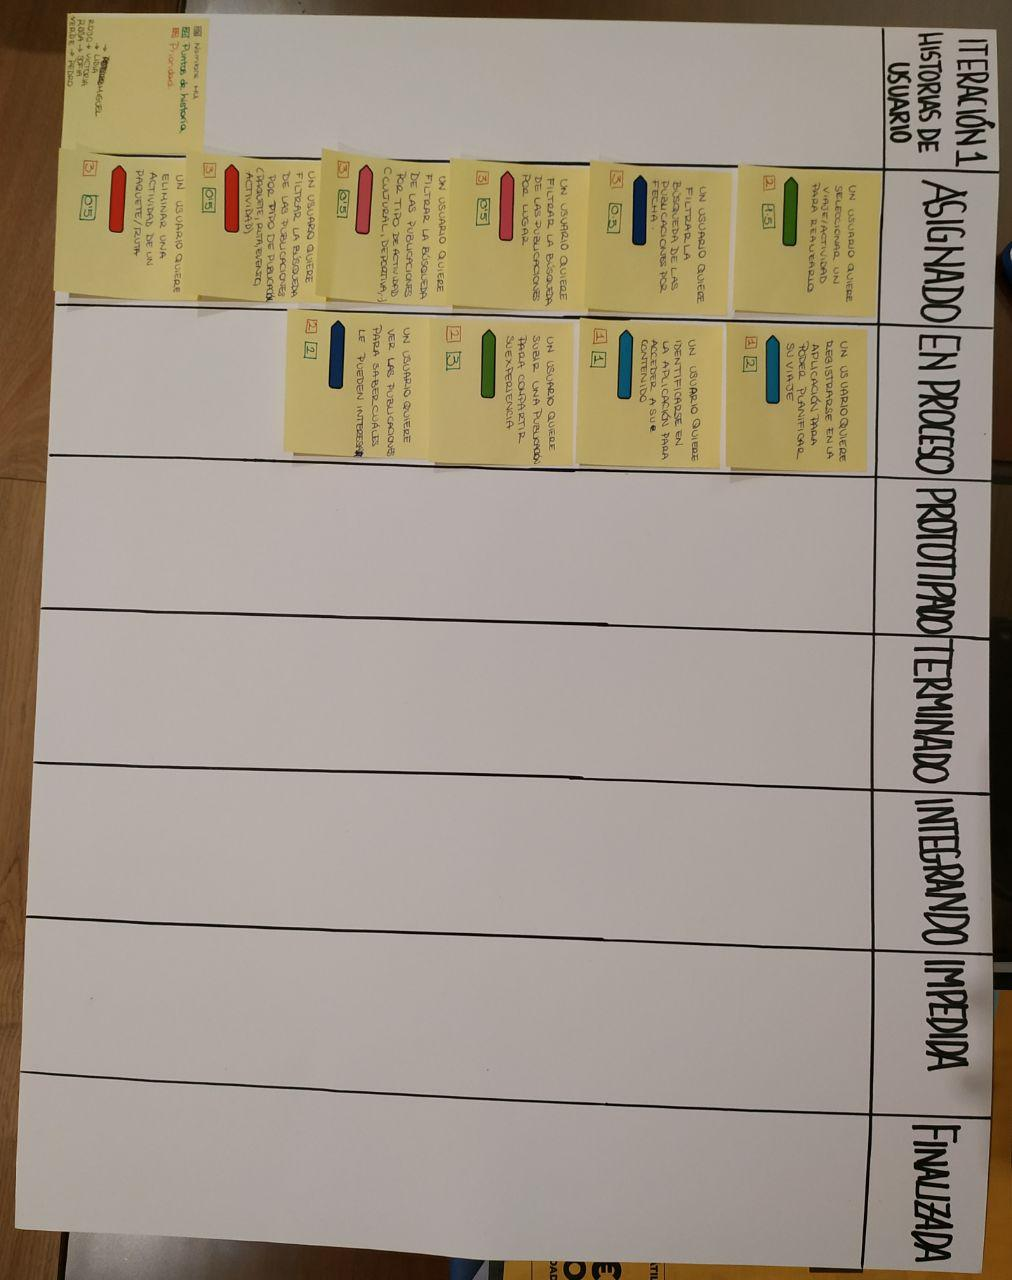
\includegraphics[angle=90, scale=0.32]{papel1_1}
	\end{center}
\end{frame}


\begin{frame}
	\begin{center}
		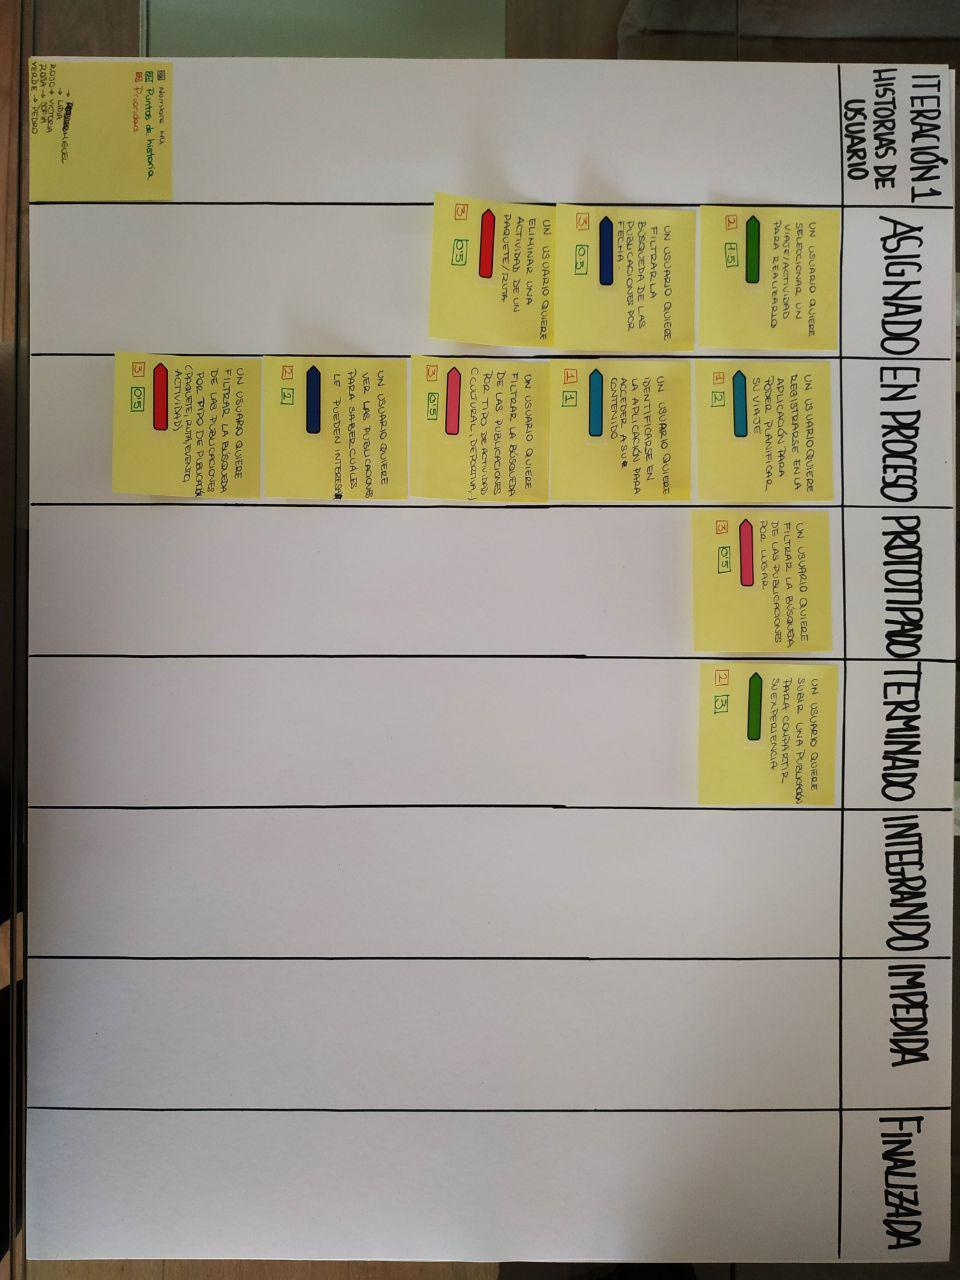
\includegraphics[angle=90, scale=0.335]{papel1_5}
	\end{center}
\end{frame}

\begin{frame}
	\begin{center}
		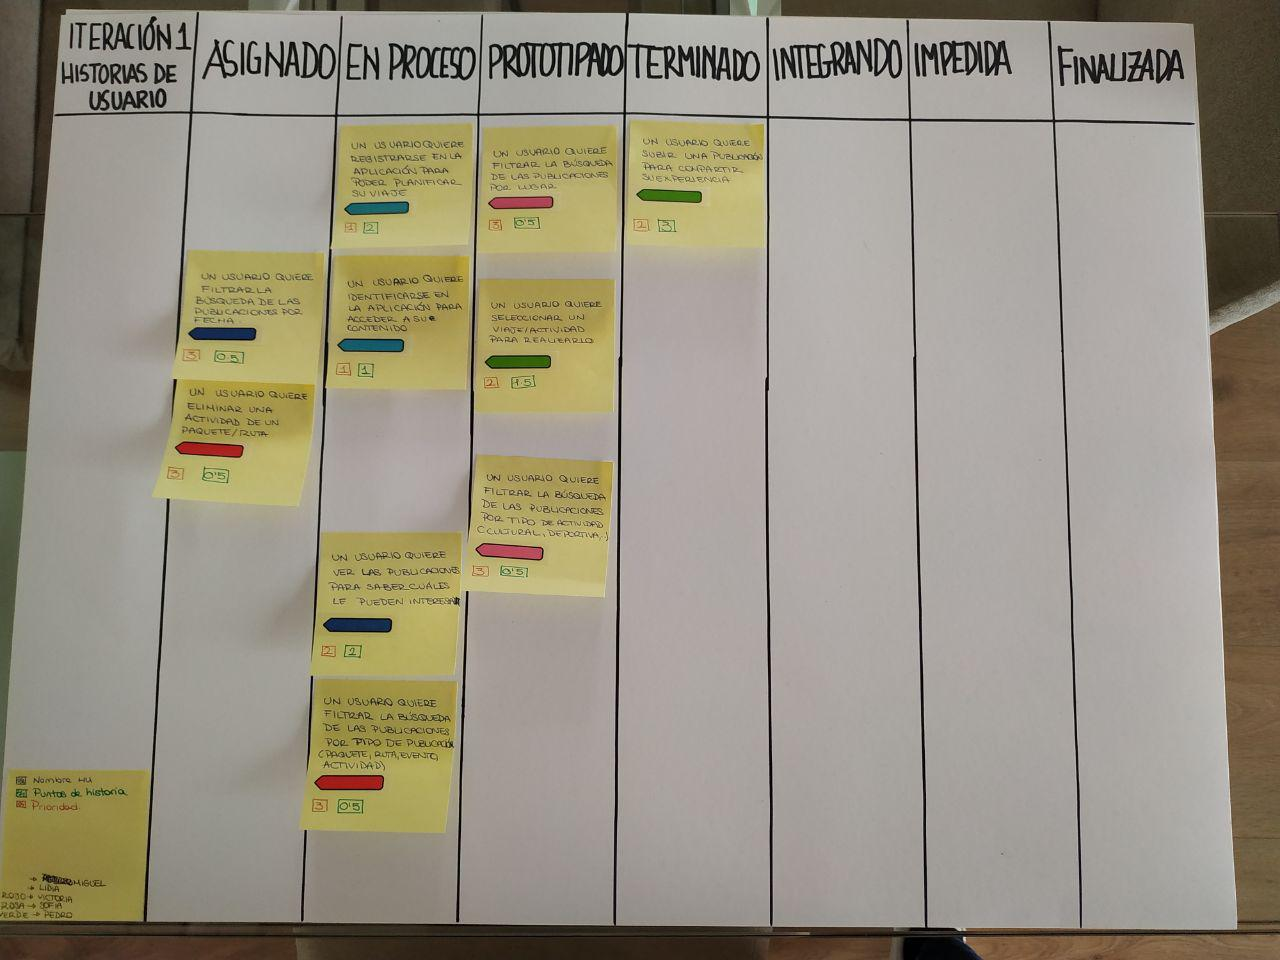
\includegraphics[angle=0, scale=0.34]{papel1_6}
	\end{center}
\end{frame}


\begin{frame}
	\begin{center}
		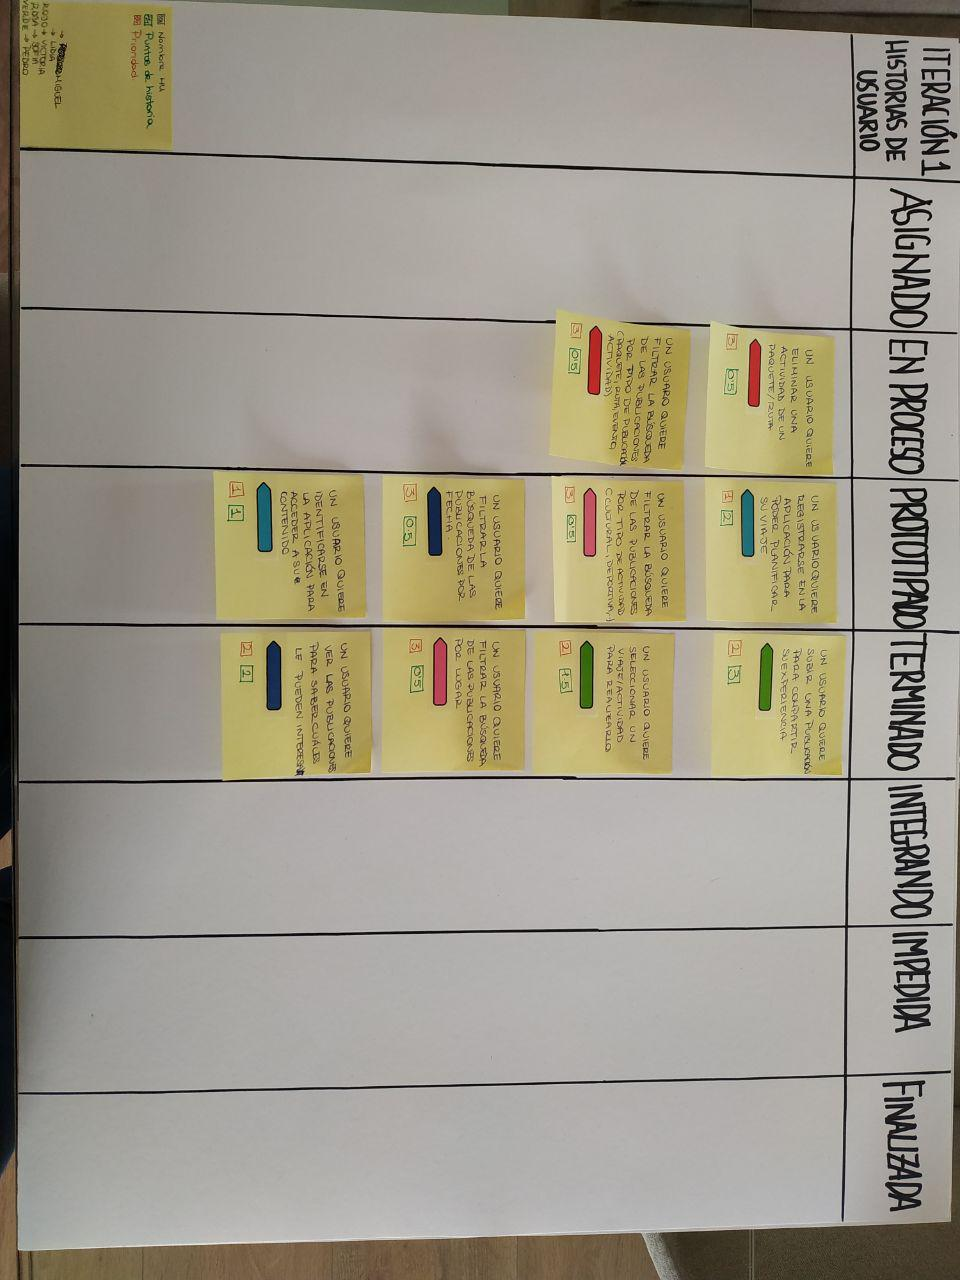
\includegraphics[angle=90, scale=0.34]{papel1_8}
	\end{center}
\end{frame}


\begin{frame}
	\begin{center}
		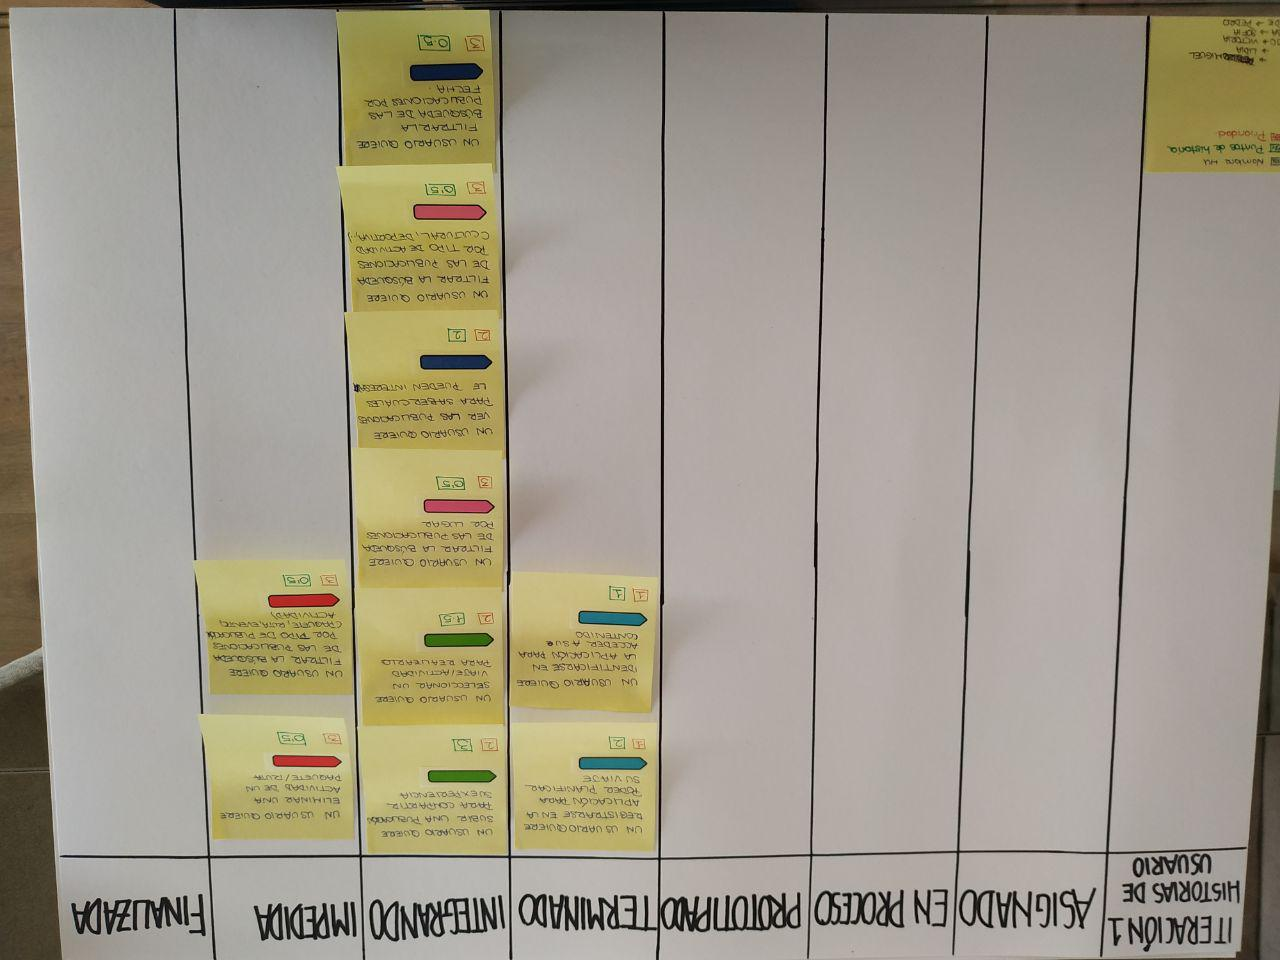
\includegraphics[angle=180, scale=0.33]{papel1_9}
	\end{center}
\end{frame}



\end{document}

